\documentclass{article}

\usepackage{lmodern}
\usepackage[T1]{fontenc}
\usepackage[spanish,activeacute]{babel}
\usepackage{mathtools}
\usepackage[utf8]{inputenc}
\usepackage{enumerate}
\usepackage[a4paper, total={7in, 10in}]{geometry}
\usepackage{graphicx}
\usepackage{charter}

\begin{document}
\begin{center}
\large \textbf{Práctica 6}: Lenguajes formales y gramáticas
\end{center}
\graphicspath{ {./img/} }
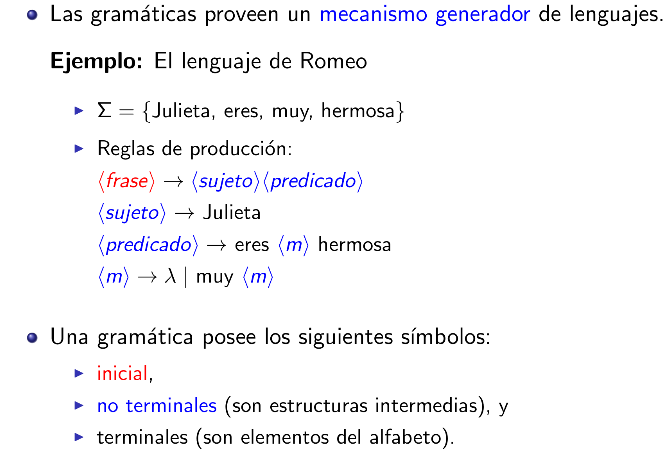
\includegraphics[scale=0.4]{1.png} \\ \\
\textbf{Definición: Gramática} es una tupla: $(N,T,P,\sigma)$ donde: \\
\begin{itemize}
  \item
    N es un conjunto finito de símbolos llamados \textbf{no terminantes}.
  \item
    T es un conjunto finito de símbolos, llamados \textbf{terminantes} o \textbf{alfabeto},
    tal que $N \cap T = \emptyset$
  \item
    P es un conjunto finito de \textbf{reglas de producción}, donde
    \[ P \subseteq ((N \cup T)^{*} - T^{*}) \times (N \cup T)^{*}\]
    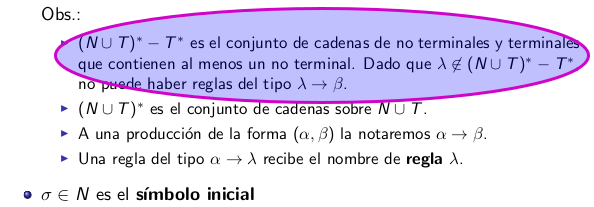
\includegraphics[scale=0.6]{4.png} \\
    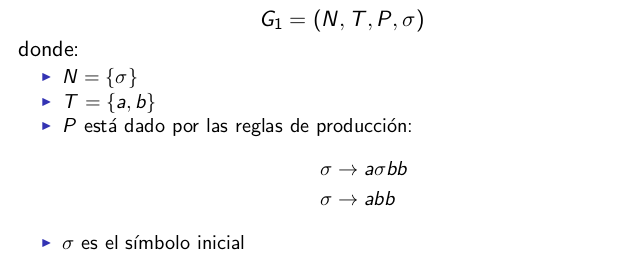
\includegraphics[scale=0.5]{5.png}
\end{itemize}
\textbf{Definición 1.} Una gramática se dice:
\begin{enumerate}[(a)]
\item
    \textit{regular} si cada producción es de la forma:
    $A \rightarrow a$ o $A \rightarrow aB$ o $A \rightarrow \lambda \quad$ 
    donde $A, B \in N$ y $a \in T$, \\ \\ \\
    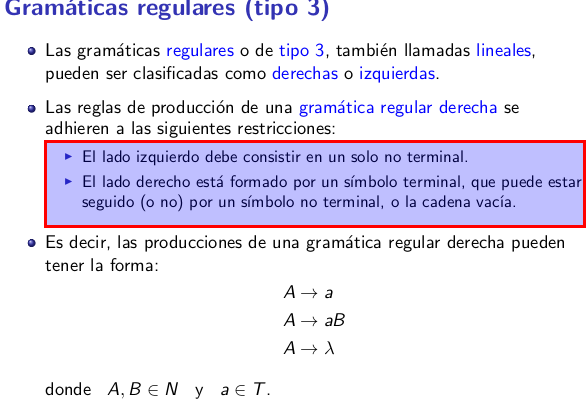
\includegraphics[scale=0.4]{3.png}
    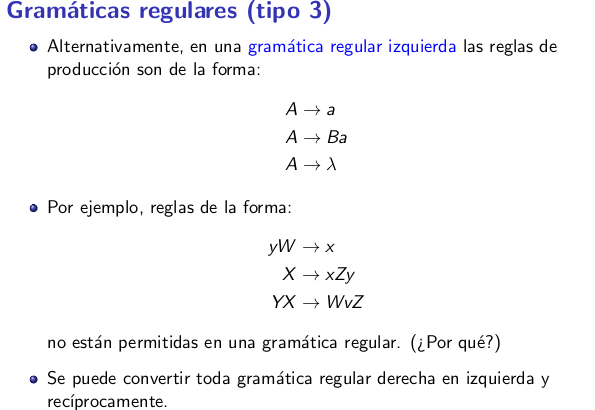
\includegraphics[scale=0.4]{2.png} \\ \\ \\ \\ \\ \\
\item
    \textit{libre} (o independiente) de contexto si cada producción es de la forma 
    $A \rightarrow \delta$ donde $A \in N$ y $\delta \in (N \cup T)^*$. \\ Otra definición: \\ 
    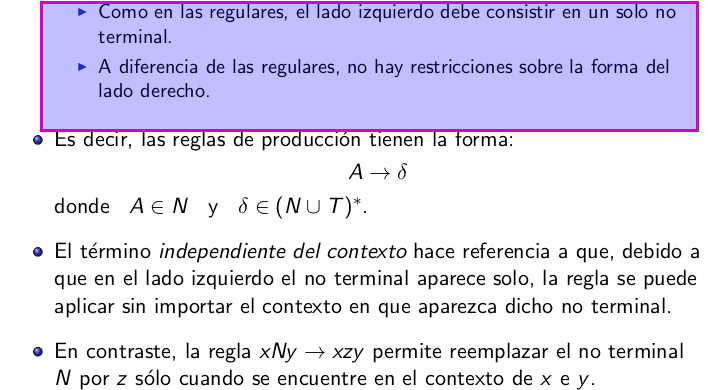
\includegraphics[scale=0.5]{6.png} \\ \\
    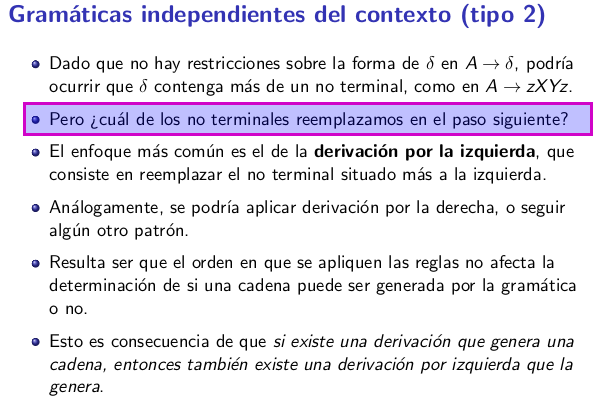
\includegraphics[scale=0.5]{7.png}
\item
  \textit{sensible al contexto} si cada producción es de la forma
    $aA\beta \rightarrow \alpha\delta\beta$ donde $A \in N, \alpha,\beta \in (N \cup T)^*$ y $\delta \in (N \cup T)^+$. \\
    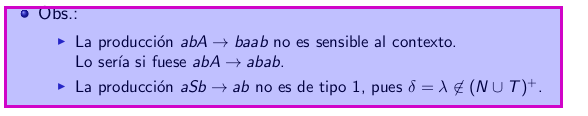
\includegraphics[scale=0.5]{8.png}
  \item
    \textit{estructurada} por frases o irrestricta si no tiene restricciones sobre la forma de sus producciones, es decir
   si son de la forma
    \[ \alpha \rightarrow \delta \text{\quad donde \quad} \alpha \in (N \cup T)^* - T^* \quad y \quad \delta \in (N \cup T)^* \]
\end{enumerate}

\begin{enumerate}[1.]
\item
Clasifique cada una de las siguientes gramáticas (dando su tipo más restrictivo):
  \begin{enumerate}[a)]
    \item
      $T = \{ a,b\}, N = \{ \sigma, A\}$, símbolo inicial $\sigma$, y producciones
      \[ \sigma \rightarrow b\sigma, \sigma \rightarrow aA, A \rightarrow a\sigma,\]
      \[ A \rightarrow bA, A \rightarrow a, \sigma \rightarrow b\]
      Regular.
    \item 
      $T = \{ a,b,c \}, N = \{ \alpha,A,B\}$, símbolo inicial $\sigma$, y producciones
      \[ \sigma \rightarrow AB, AB \rightarrow BA, A \rightarrow aA,\]
      \[ B \rightarrow Bb, A \rightarrow a, B \rightarrow b\] \\
       Sensible al contexto.
    \item
      $T = \{ a,b\}, N = \{ \sigma, A,B\}$, śimbolo inicial $\sigma$ y producciones:
      \[ \sigma \rightarrow A, \quad \sigma \rightarrow AAB,\quad Aa \rightarrow ABa, \quad A \rightarrow aa,\]
      \[ Bb \rightarrow ABb, \quad AB \rightarrow ABB, \quad B \rightarrow b.\]
      Sensible al contexto.
    \item
      $T = \{ a,b,c \}, N = \{\sigma,A,B \},$ símbolo inicial $\sigma$, y producciones:
      \[ \sigma \rightarrow BAB, \quad \sigma \rightarrow ABA, \quad A \rightarrow AB, \quad B \rightarrow BA,\]
      \[A \rightarrow aA, \quad A ab, \quad B \rightarrow b.\]
      Independiente de contexto (libre).
  \end{enumerate}
\item
  Dé una derivación de las sigueintes cadenas en las gramáticas especificadas:
    \begin{enumerate}[a)]
      \item 
        Cadena $bbabbab$ en la gramática \textit{1a}.
        \[ \sigma \]
        \[ = < \sigma \rightarrow b\sigma >\]
        \[ b\sigma \]
        \[ = < \sigma \rightarrow b\sigma > \]
        \[ bb\sigma \]
        \[ = < \sigma \rightarrow aA > \]
        \[ bbaA \]
        \[ = < A \rightarrow bA > \]
        \[ bbabA \]
        \[ = < A \rightarrow bA > \]
        \[ bbabbA \]
        \[ = <A \rightarrow a\sigma> \]
        \[ bbabba\sigma\]
        \[ = <\sigma \rightarrow b> \]
        \[ bbabbab. \]
      \item
        Cadena $abab$ en la gramática \textit{1b}.
        \[ \sigma \]
        \[ = < \sigma \rightarrow AB> \]
        \[ AB \]
        \[ = <A \rightarrow aA, B \rightarrow Bb>\]
        \[ aABb \]
        \[ = < AB \rightarrow BA > \]
        \[ aBAb \]
        \[ = <A \rightarrow a, B \rightarrow b> \]
        \[ abab. \] 
      \item
        \[ \sigma \]
        \[ = < \sigma \rightarrow AAB > \]
        \[ AAB \]
        \[ =< B \rightarrow b > \]
        \[ AAb \]
        \[ = < A \rightarrow aA > \]
        \[ Aaab \]
        \[ = < Aa \rightarrow ABa > \]
        \[ ABaab \]
        \[ = <B \rightarrow b> \]
        \[ Abaab \]
        \[ =<A \rightarrow aa> \]
        \[ aabaab \]
      \item
        \[ \sigma \]
        \[ = < \sigma \rightarrow ABA >  \]
        \[ ABA \]
        \[ = < A \rightarrow AB \]
        \[ ABAB \]
        \[ = <B \rightarrow b > \]
        \[ ABAb \]
        \[ = <A \rightarrow ab > \]
        \[ ABabb \]
        \[ = < B \rightarrow b> \]
        \[ Ababb \]
        \[ = < A \rightarrow ab >  \]
        \[ abbabb \]
    \end{enumerate}
  \item 
    Muestre que la cadena $abbbabaaba$ no está en el lenguaje generado por la gramática $G = (N,T,P,\sigma)$,
    donde $N = \{ \sigma, A, B \}$, $T= \{ a,b \}$, símbolo inicial $\sigma$ y producciones: 
    \[ \sigma \rightarrow aaBA, \quad \sigma \rightarrow ABB, \quad A \rightarrow aaB, \quad A \rightarrow \lambda \]
    \[ aBa \rightarrow A, \quad Aaa \rightarrow B, \quad B \rightarrow AabaB, \quad B \rightarrow bbb \]

    Ya sea, comenzando con $\sigma \rightarrow aaBA$, o $\sigma \rightarrow ABB$, al aplicar cualquiera de las reglas
    de producción posibles, siempre se llega a algo con final en B o bbb. Este final es imposible de cambiar por a.
    Por lo tanto $abbbabaaba$ no está en dicho lenguaje.
  \item
    Dé una gramaica del tipo pedido que genere los siguientes lenguajes:
    \begin{itemize}
      \item
        Gramática regular:
        \begin{enumerate}[i.]
          \item
            Cadenas sobre el alfabeto $\{ a,b \}$ que comiencen con a.
          \item
            Cadenas sobre el alfabeto $\{ a,b \}$ que contengan exactamente una a y terminen con al menos
            una b.
          \item
            Cadenas sobre el alfabeto $\{ a,b\}$ que terminen con $ba$.
          \item
            Cadenas sobre el alfabeto $\{a,b\}$ que contengan $ba$.
          \item
            Cadenas sobre el alfabeto $\{a,b\}$ que no terminen con $ab$.
        \end{enumerate}
      \item
        \begin{enumerate}
          \item
            Cadenas sobre el alfabeto $\{a,b\}$ de la forma $a^n b^n$ para $n \geq 0$.
          \item
            Cadenas s
        \end{enumerate}
    \end{itemize}
  \item
    Sea $\mathcal{L}$ el ocnjunto de cadenas sobre $\{a,b\}$ que contienen la misma cantidad de símbolos
    a y b. Analice si cada una de las siguientes gramáticas genera $\mathcal{L}$. En caso negativo, dé un
    contraejemplo (es decir, una cadena generada por la gramática pero que no está en $\mathcal{L}$, o
    una cadena que está en $\mathcal{L}$ pero no es generada por la gramática). En todas las gramáticas el
    símbolos inicial es S.

    \begin{enumerate}[a)]
      \item
        $S \rightarrow aSb | bSa | \lambda$
    \end{enumerate} 
  \item
    \begin{enumerate}[i.]
      \item
        Muestre que si cada producción de una gramática G es de la forma.
        \[ A \rightarrow \quad o \quad A \rightarrow \alpha B \quad o \quad A \rightarrow \lambda \quad \text{donde} 
        \quad A,B \in N \quad y \quad \alpha \in T^{+} \]
        entonces existe una gramática regular $G'$ equivalente (es decir, tal que $L(G') = L(G))$.
      \item
        Aplique el apartado anterior para modificar la gramática siguiente (símbolo inicial: S) de manera de formar
        una gramática regular equivalente.
        \[ S \rightarrow yX \]
        \[ X \rightarrow xxX \]
        \[ X \rightarrow yY \]
        \[ Y \rightarrow \lambda \]
        \[ A \rightarrow xX \]
    \end{enumerate}
  \item
    Muestre que un lenguaje regular que no contiene a $\lambda$ puede ser generado por una gramática que no contiene
    reglas de la forma $A \rightarrow \lambda$. \\ \\
    \textbf{Definición 2}. Una gramática se dice que está en forma normal de Chomsky sii toda producción es de la forma
    \[ A \rightarrow BC \quad o \quad A \rightarrow a \quad o \quad S \rightarrow \lambda \]
    donde $A,B,C \in N, a \in T, S$ es el no terminal inicial y $B$ y $C$ son distintos de $S$.
  \item
    Convertir a la forma normal de Chomsky:
    \[ S \rightarrow xSy \]
    \[ S \rightarrow wNz \]
    \[ N \rightarrow S\]
    \[ N \rightarrow \lambda \]

    $G = (N,T,P,S)$ \\
    $N = \{ A,B,C,X,Y,W,Z \}$ \\
    $T = \{ x,y,w,z \}$ \\ \\
    P está dado por las siguientes reglas de producción: \\ \\
    $\quad \begin{array}{lcl}
      S \rightarrow XA\\
      S \rightarrow WB \\
      A \rightarrow SY
     \end{array} \quad
    \begin{array}{lcl}
      B \rightarrow NZ \\
      C \rightarrow S \\
      C \rightarrow \lambda
    \end{array} \quad
    \begin{array}{lcl}
      X \rightarrow x \\
      Y \rightarrow y \\
      W \rightarrow w \\
      Z \rightarrow z
    \end{array}$
  \item
    \begin{enumerate}[i.]
      \item
        Se puede probar que el lenguaje $\mathcal{L} = \{ a^n b^n c^n | n \in \mathcal{N} \}$ no es independiente
        de contexto. Usando este resultado probar que el conjunto de los lenguajes independientes de contexto no 
        es cerrado bajo la opración de intersección, hallando dos lenguajes que sean independientes de contexto
        cuya intersección sea $\mathcal{L}$.
      \item
        Probar que el conjunto de los lenguajes independientes de contexto no es cerrado bajo la operación de complemento.
    \end{enumerate}
  \item
    Se puede probar que la intersección de un lenguaje independiente del contexto y uno regular es independiente de contexto.
    Usar este resultado y el enunciado del ejercicio 9a para probar que el lenguaje $\{ w\in \{a,b,c \}^* | N_a(w) = 
    N_b(w) = N_c(w) \}$ no es independiente del contexto.
\end{enumerate}


\end{document}
